%!TEX root = thesis.tex
\chapter{Summary, conclusions, and future work}

\section{Summary and conclusions}
Confining ordered materials can lead to interesting phenomonology due to the interplay between the order and the confinement geometry.
For the nematic materials used in this Thesis, it is often the curvature of the confining volume or surface that affects the nematic order.
This is a consequence of the fact that nematic materials possess only orientational order; with the order defined by the director $\mathbf{n}$, the free energy has order $|\nabla \mathbf{n}|^2$, indicating that curvature in the director field costs energy.
The influence of curvature on a nematic material is even more explicit when considering a 2D nematic constrained to lie on a surface.
In this situation, the free energy can be written to resemble that of a plasma, with defects in the nematic acting like discrete charges in the plasma and the Gaussian curvature of the surface as background charge in the plasma  [see Eq~\ref{e:1-TopTheoryofDefects}].
Thus, if the surface has both positive and negative Guassian curvature and the nematic has both positive and negative defects, the defects are predicted to segregate, with the positive defects migrating to the regions of positive Gaussian curvature and vice versa.

We explore this situation experimentally using an active polymeric nematic depleted to the surface of a toroidal droplet.
Due to the activity, the nematic is filled with pairs of constantly creating and annihilating $s = \pm 1/2$ defects, with the $s = +1/2$ defects acting as self-propelled particles driving the nematic into a turbulent state.
We measure the time-averaged topological charge in regions on the toroidal droplet and find that the average charge varies linearly with the integrated Gaussian curvature in the region.
The slope of this relationship is positive, indicating that our system exhibits defect unbinding.
In contrast to predictions for a system at equilibrium, we find that the active unbinding depends only on the local geometry and is insensitive to the size and aspect ratio of our toroidal droplets.
Comparing our experimental results to a numerical integration of the equations of motion of active nematic defects further illustrates that the defect unbinding also depends on the defect number density, and that the unbinding can even be suppressed in the limit of high activity.
Finally, by using topological defects as micro-rheological tracers and quantitatively comparing our experimental and theoretical results, we are able to estimate the Frank elastic constant, the active stress, and the defect mobility of a microtubule-kinesin active NLC.

Overall, our results not only confirm the theory of topological defects on curved surfaces, but also demonstrate how adding activity to an ordered material changes and enriches equilibrium expectations.
For example, because the active unbinding is driven solely by local interactions, we see that a combination of activity and curvature can be used to guide defects in ordered materials.
In addition, our work introduces a new avenue for the quantitative mechanical characterization of active fluids.

So far we have only examined the behavior of the average topological charge $\overbar{s}_{\Theta} = (\overbar{N}^{+}_{\Theta} - \overbar{N}^{-}_{\Theta})/2$, with $\overbar{N}^{\pm}_{\Theta}$ the time-averaged number of $s = \pm1/2$ defects in a region $\Theta$ on the active nematic toroid.
This is only one of the things that our setup can explore.
For example, we have preliminary data showing the time-averaged number density $\overbar{N}_{\Theta}/A_{\Theta} = (\overbar{N}^{+}_{\Theta} + \overbar{N}^{-}_{\Theta})/A_{\Theta}$ depends on not only the local curvature, but also the aspect ratio of the toroid.
It is not clear why the topological charge depends only on local interactions while the defect number density depends on the size and shape of the toroidal droplet.
In addition, there is work with this active nematic system in flat space showing that the $s = +1/2$ defects can themselves assemble to form a nematic phase, where $S$ associated to this higher-order nematic phase grows as $\overbar{N}_{\Theta}$ grows.
However, our preliminary data suggest that on a toroid, the $s = +1/2$ defects do not form a nematic phase but instead a polar phase, and that the strength of this polar phase grows as the $\overbar{N}_{\Theta}$ decreases.
These are just two examples of future directions that we are currently working on that further explore the role of curvature and activity in partially ordered matter.

We also consider a NLC confined to toroidal droplets and bent capillaries under homeotropic boundary conditions.
We observe spontaneous reflection symmetry breaking due to a twist distortion relieving the energetic cost of two competing bend distortions.
The competition between the distortions is given by the local aspect ratio, $\xi$, comparing the radii of curvature of the two bend distortions.
Thus, $\xi$ also governs the amount of twist in the system, with the twist decreasing with increasing $\xi$.
This geometrically-tuned chirality is similar to previous results in our group with NLC confined to toroidal droplets with degenerate planar anchoring, showing that tuning a ratio of curvatures to control chirality in NLC does not depend on the anchoring.

Lastly, we explore the equilibrium defect structure in NLC confined to capillary bridges under homeotropic boundary conditions.
We find that the defect structure in our bridges depends on both the shape of the bounding surface as well as the aspect ratio of the bridge.
The aspect ratio determines whether the bridge contains a ring defect or a point defect, and the boundary shape determines whether the defect is radial or hyperbolic, with waist-like shapes containing hyperbolic defects and barrel-like shapes containing radial defects.
In addition, we find that in a waist structure the point defect can be metastable, causing the transition between a ring defect and a point defect to exhibit hysteresis.
We compare with numerical calculations and find good agreement with our experiments.
Our work thus shows that shape can be used to influence and control the equilibrium defect states in confined NLC under homeotropic boundary conditions.
Interestingly, the numerical calculations predict that a cylinder-like structure can have defect transitions between radial rings and hyperbolic points as well as between radial rings and hyperbolic rings.
The specific pathways for these transitions are unclear and would be an interesting direction for future work.

\section{Defect orientation on curved surfaces: current status}
Prior work with a microtubule-kinesin active nematic on a flat surface demonstrated that the $s = +1/2$ defects self-organize into a higher-order nematic phase~\cite{RN27}.
The orientation of each $s = +1/2$ defect is given by its velocity; calculating $\mathbf{Q}$ for a collection of defect orientations uncovers long-range nematic order~\cite{RN27}.
The strength of the order increases with increasing defect density and this higher-order nematic is typically defect-free, with a homogeneous director over the entire sample~\cite{RN27}.
We are currently investigating how the $s = \pm 1/2$ defect orientations couple to the curvature of our toroidal droplets.


\subsection{Theory}
The velocity of the $s = +1/2$ defects is not the only way to assign an orientation to each defect.
Recent work showed that the polar structure of the $s = +1/2$ defect can be characterized by a vector, and that the distortion free energy of a pair of $s = +1/2$ defects is minimized when the orientation vectors are antiparallel~\cite{RN6}.
Thus, a dense collection of $s = +1/2$ defects would minimize its free energy by aligning antiparallel to each other, forming a higher-order nematic phase.
For a single $s = +1/2$ defect, this orientation $\mathbf{p}$ is calculated by:
\begin{equation}
  p_i = \left \langle \partial_j Q_{ij}^{(\alpha)} \right \rangle_{\alpha},\label{e:7-LGpositive}
\end{equation}
where $Q_{ij}$ is the tensor order parameter and the average is taken along a closed contour encircling the defect.
Reference~\cite{RN6} also proposed a method to characterize the orientation of $s = -1/2$ disclinations; however, their method requires a coordinate basis to be chosen.

Alternately, Ref.~\cite{jsel} has a method to calculate disclination orientation by constructing tensors of the appropriate rank.
For example, the orientations of $s = +1/2$ and $s = -1/2$ disclinations are calculated via:
\begin{align}
    b_i &= \left \langle \partial_j (n_{i}^{(\alpha)}n_{j}^{(\alpha)}) \right \rangle_{\alpha},\label{e:7-JSpositive} \\
    T_{ijk} &= \left \langle \partial_i (n_{j}^{(\alpha)}n_{k}^{(\alpha)}) + \partial_j (n_{i}^{(\alpha)}n_{k}^{(\alpha)}) + \partial_k (n_{i}^{(\alpha)}n_{j}^{(\alpha)}) \right \rangle_{\alpha},\label{e:7-JSnegative}
\end{align}
respectively, where the average is again taken over a path encircling the disclination.
Importantly, the orientations of the $s = \pm 1/2$ disclinations calculated via Eqs.~\ref{e:7-JSpositive}~and~\ref{e:7-JSnegative} are both tensors; they do not depend on the choice of a coordinate basis.
\begin{figure}
  \centering
  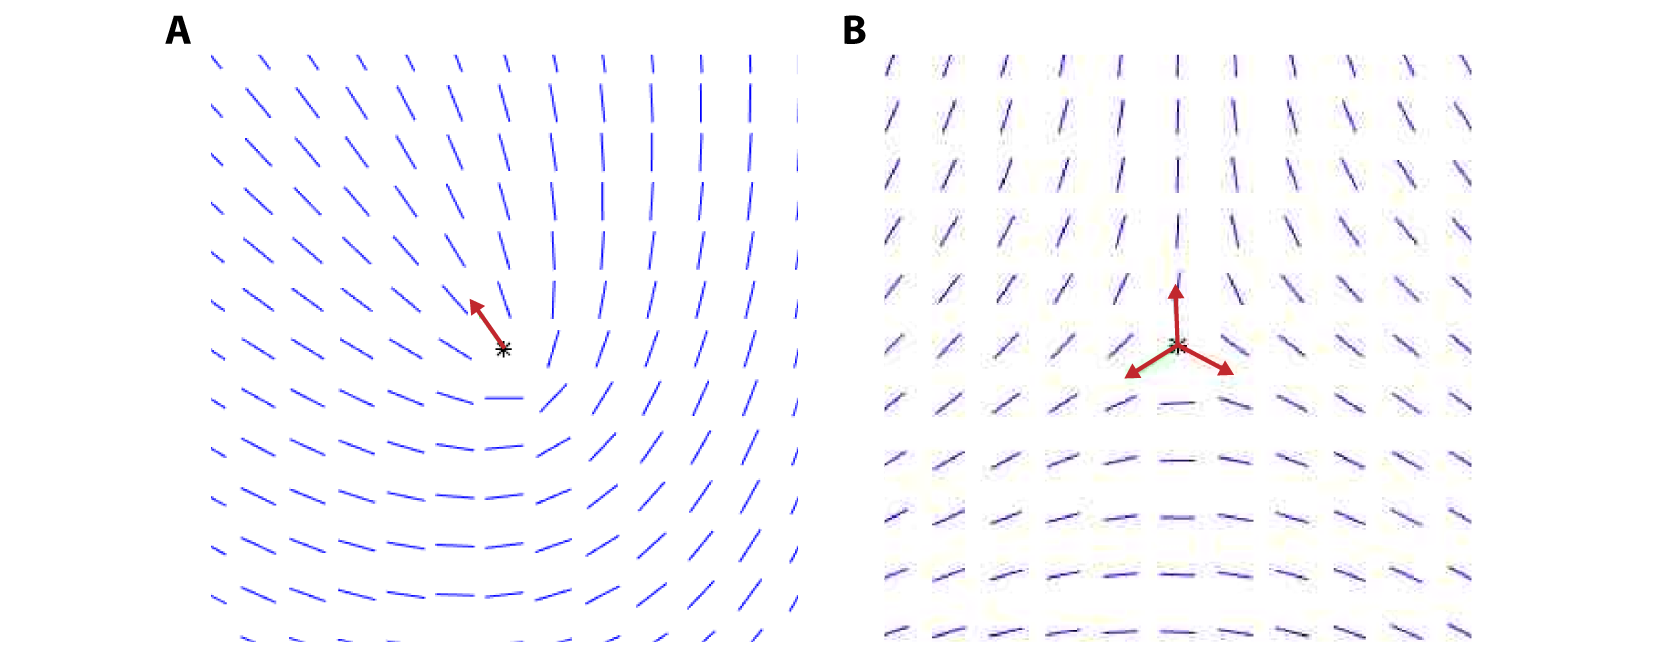
\includegraphics{figures/C7/Ch7-Figs_BasicOrients.png}
  \caption{Example director fields and axes of symmetry for an (A) $s = +1/2$ and an (B) $s=-1/2$ defect.
  The axes of symmetry were calculated with Eqs.~\ref{e:7-JSpositive}~and~\ref{e:7-JSnegative}.
  }\label{f:7-BasicOrients}
\end{figure}

Comparing the two methods to calculate the orientation of an $s = +1/2$ disclination, we have:
\begin{align}
 p_i &= \left \langle \partial_j Q_{ij}^{(\alpha)} \right \rangle_{\alpha} \nonumber \\
  &= \left \langle \partial_j \bigg(S^{(\alpha)}\bigg(n_{i}^{(\alpha)}n_{j}^{(\alpha)} - \frac{1}{2}\delta_{ij}\bigg)\bigg) \right \rangle_{\alpha} \nonumber \\
  &= \left \langle (\partial_j S^{(\alpha)}) \bigg(n_{i}^{(\alpha)}n_{j}^{(\alpha)} - \frac{1}{2}\delta_{ij}\bigg) \right \rangle_{\alpha}
      + \left \langle S^{(\alpha)} \partial_j (n_{i}^{(\alpha)}n_{j}^{(\alpha)}) \right \rangle_{\alpha} \nonumber \\
  &= \left \langle \frac{\partial_j S^{(\alpha)}}{S^{(\alpha)}} Q_{ij}^{(\alpha)}\right \rangle_{\alpha}
      + \left \langle S^{(\alpha)} \partial_j (n_{i}^{(\alpha)}n_{j}^{(\alpha)}) \right \rangle_{\alpha}\label{e:7-comparison}.
\end{align}
If we choose a contour where $S$ is constant, Eq.~\ref{e:7-comparison} becomes
\begin{equation}
  p_i = S \, b_i.
\end{equation}
Under this condition, both approaches give the same orientation.
However, in general, Eq.~\ref{e:7-LGpositive} includes additional information about the spatial variation of $S$ near the disclination.
Since the methodology in Ref~\cite{jsel} produces a tensor for both $s = \pm 1/2$ disclinations, we will use Eqs.~\ref{e:7-JSpositive}~and~\ref{e:7-JSnegative} to calculate our defect orientations.


\subsection{Experiment}
Our goal is to examine the defect orientations on the curved surface of our toroidal droplets.
However, we project our data from the surface of the toroid onto a plane, forming a 2D image from which we determine the director and the defects.
Thus, we will find the defect orientations in the 2D image and then project the defect orientations back onto our toroidal surface.
In the plane of the image, we have the Cartesian coordinate system $\{ \hat{x},\hat{y},\hat{z} \}$ with unit vectors $(1,0,0)$, $(0,1,0)$, and $(0,0,1)$, respectively.
For an arbitrary unit surface normal $\mathbf{k} = (a, b, \sqrt{1-a^2-b^2})$, we define $\hat{v} = \hat{k} \times \hat{x}/|\hat{k} \times \hat{x}|$ and $\hat{u} = \hat{v} \times \hat{k}$, giving us an orthonormal coordinate frame on the surface $\{\hat{u},\hat{v},\hat{k} \}$.

Transforming between $\mathbf{r} \in \mathbb{R}^2$ to $\mathbf{r}'$ on the surface of our toroid,
\begin{equation}
  \mathbf{r}' =
  \begin{pmatrix}
  \frac{1}{\sqrt{1-a^2}} & 0 \\
  \frac{ab}{\sqrt{(1-a^2)(1-a^2-b^2)}} & \sqrt{\frac{1-a^2}{1-a^2-b^2}}
  \end{pmatrix}
  \mathbf{r} = \bm{H}\mathbf{r}.
\end{equation}
However, since $\{ \hat{u},\hat{v}\}$ depends on $\hat{k}$, $\{ \hat{u},\hat{v}\}$ will change over the surface of our droplet, making it difficult to compare defect orientations between different points on the surface.
Instead, we will record our defect orientations on the surface of the torus in terms of a pair of curvilinear coordinate systems.
The first coordinate system is the standard toroidal coordinate system, $\{\hat{\theta}, \hat{\varphi}, \hat{r}  \}$, where $\hat{r} = \mathbf{k}$, the surface normal.
The second coordinate system is $\{\hat{\theta}', \hat{\varphi}',\mathbf{k} \}$, with $\hat{\theta}' = (\nabla K)/|\nabla K|$, and $\hat{\varphi}' = \mathbf{k} \times \hat{\theta}'$.
For a perfect toroid, the two coordinate systems are equivalent; however, in our case, the surface can be rough and our droplets are not perfectly axisymmetric.
Thus, our two coordinate systems should allow us to distinguish between global effects driven by the toroidal geometry and local effects driven by $K$.

To calculate $\hat{\theta}$ and $\hat{\varphi}$, we start by finding the central circle from our data in $\mathbb{R}^2$.
We fit circles to the outer and inner contours in the 2D image of the toroidal droplet and average these contours to get an estimate of the central circle of our toroidal droplet.
From the central circle, we can define a set of polar coordinates in the image $\{\hat{\rho}, \hat{\phi}\}$.
We project $\hat{\phi}$ onto the surface of the torus to yield $\bm{\varphi} = \bm{H}\hat{\phi}$, and then normalize to get $\hat{\varphi} = \bm{\varphi}/|\bm{\varphi}|$.
Finally, we calculate $\hat{\theta} =  \hat{\varphi} \times \mathbf{k}$ to obtain the standard toroidal coordinate system on our toroidal droplet.

To calculate $\hat{\theta}'$ and $\hat{\varphi}'$, we start by computing $\nabla K$ in the 2D image and projecting it to the surface of the toroid to get:
\begin{equation}
  \bm{\theta}' =
  \begin{pmatrix}
    \sqrt{1-a^2} & -\frac{ab}{\sqrt{1-a^2}} \\
    0 & \sqrt{\frac{1-a^2-b^2}{1-a^2}}
  \end{pmatrix}
  \nabla K = \bm{H}^{-1} \nabla K.
\end{equation}
Normalizing, we get $\hat{\theta}' = \bm{\theta}'/|\bm{\theta}'|$, and then calculate $\hat{\phi}' = \mathbf{k} \times \hat{\theta}'$.
Note that we project $\nabla K$ from the image to the surface of the toroid using $\bm{H}^{-1}$; $\nabla K$ is a covector and thus the transformation matrix is the inverse of that for a vector.

As a first attempt, we will bin the surface by $K$ and compute the order parameters in each bin.
We will use overlapping bins of constant area in the 2D image.

We start by choosing a binsize $N$, in pixels.
For a total area, $A$, in pixels, in the 2D image of the toroid, we consider a total of $A-N$ bins.
With this protocol, two adjacent bins share all but a single pixel.
We characterize each bin with $\langle K \rangle$, and then calculate the relevant order parameters in the bin using all $s = \pm 1/2$ defects in the bin over all time frames.
For the $s = +1/2$ disclinations, we calculate the polar and nematic order parameters
\begin{align}
  S_{polar} \bm{\nu} &= \frac{1}{n} \sum\limits_{\alpha=1}^n \mathbf{b}^{(\alpha)},\label{e:7-polarorder} \\
  \mathbf{Q} &= S_{nem} \left (\mathbf{n} \otimes \mathbf{n} \right ) - \frac{1}{2}\mathbb{1} = \frac{1}{n} \sum\limits_{\alpha=1}^n \mathbf{b}^{(\alpha)} \otimes \mathbf{b}^{(\alpha)} - \frac{1}{2}\mathbb{1}\label{e:7-nematicorder},
\end{align}
where $S_{polar}$ and $S_{nem}$ is the magnitude of the order and $\bm{\nu}$ and $\mathbf{n}$ unit vectors describing the direction of the order, for polar order and nematic order, respectively.
We note that Eq.~\ref{e:7-nematicorder} is equivalent to Eq.~\ref{e:2-2DOrderRaw} and Eq.~\ref{e:2-2DOrderDiag}.

For the $s = -1/2$ disclinations, we take the orientation of $T_{ijk}$ to be the angle $\phi_0 \in [-\pi/3,\pi/3)$, the orientation of one of the three axes of symmetry of an $s = -1/2$ disclination.
Consider $\mathbf{n} = (n_x \hat{x}, n_y \hat{y})$ surrounding an $s = -1/2$ disclination, where $\theta = \arctan (y/x)$ is the polar angle describing the position.
Then, if $\phi = \theta + \phi_0$ describes the director orientation, we can write the director field surrounding the disclination as $\mathbf{n} = (\cos(\phi/2)\hat{x},-\sin(\phi/2)\hat{y})$.
Computing $T_{ijk}$ according to Eq.~\ref{e:7-JSnegative} and averaging over all $\theta$, we have:
 \begin{align}
   \langle T_{ij1}(\theta) \rangle_{\theta} &=
        \frac{3}{4}\begin{pmatrix}
          \cos \phi_0 & -\sin \phi_0 \\
          -\sin \phi_0 & -\cos \phi_0
        \end{pmatrix}\nonumber \\
  \langle T_{ij2}(\theta) \rangle_{\theta} &=
       \frac{3}{4}\begin{pmatrix}
         -\sin \phi_0 & -\cos \phi_0 \\
         -\cos \phi_0 & \sin \phi_0
       \end{pmatrix}\label{e:7-TijkBIG}
 \end{align}
From Eq.~\ref{e:7-TijkBIG}, we can now obtain $\phi_0$ from $\langle T_{ijk}(\theta) \rangle_{\theta}$ via:
\begin{equation}\label{e:7-phi0Calc}
  \phi_0 = \arctan \left ( \frac{\langle T_{222}(\theta) - T_{121}(\theta) - T_{112}(\theta) - T_{211}(\theta)  \rangle_{\theta}} {\langle T_{111}(\theta) - T_{221}(\theta) - T_{122}(\theta) - T_{212}(\theta)  \rangle_{\theta}} \right).
\end{equation}

Now, we use $\phi_0$ to calculate the bond-angle order parameter for three-fold symmetry for the $s = -1/2$ disclinations in the bin
\begin{equation}\label{e:7-hexorder}
  S_{bond} \exp(i 3 \Phi_o) = \frac{1}{n}\sum\limits_{\alpha = 1}^n \exp (i 3 \phi_o^{(\alpha)}),
\end{equation}
where $S_{bond}$ is the magnitude of the order and $\Phi_o$ is an angle giving the orientation of the order.
\begin{figure}
  \centering
  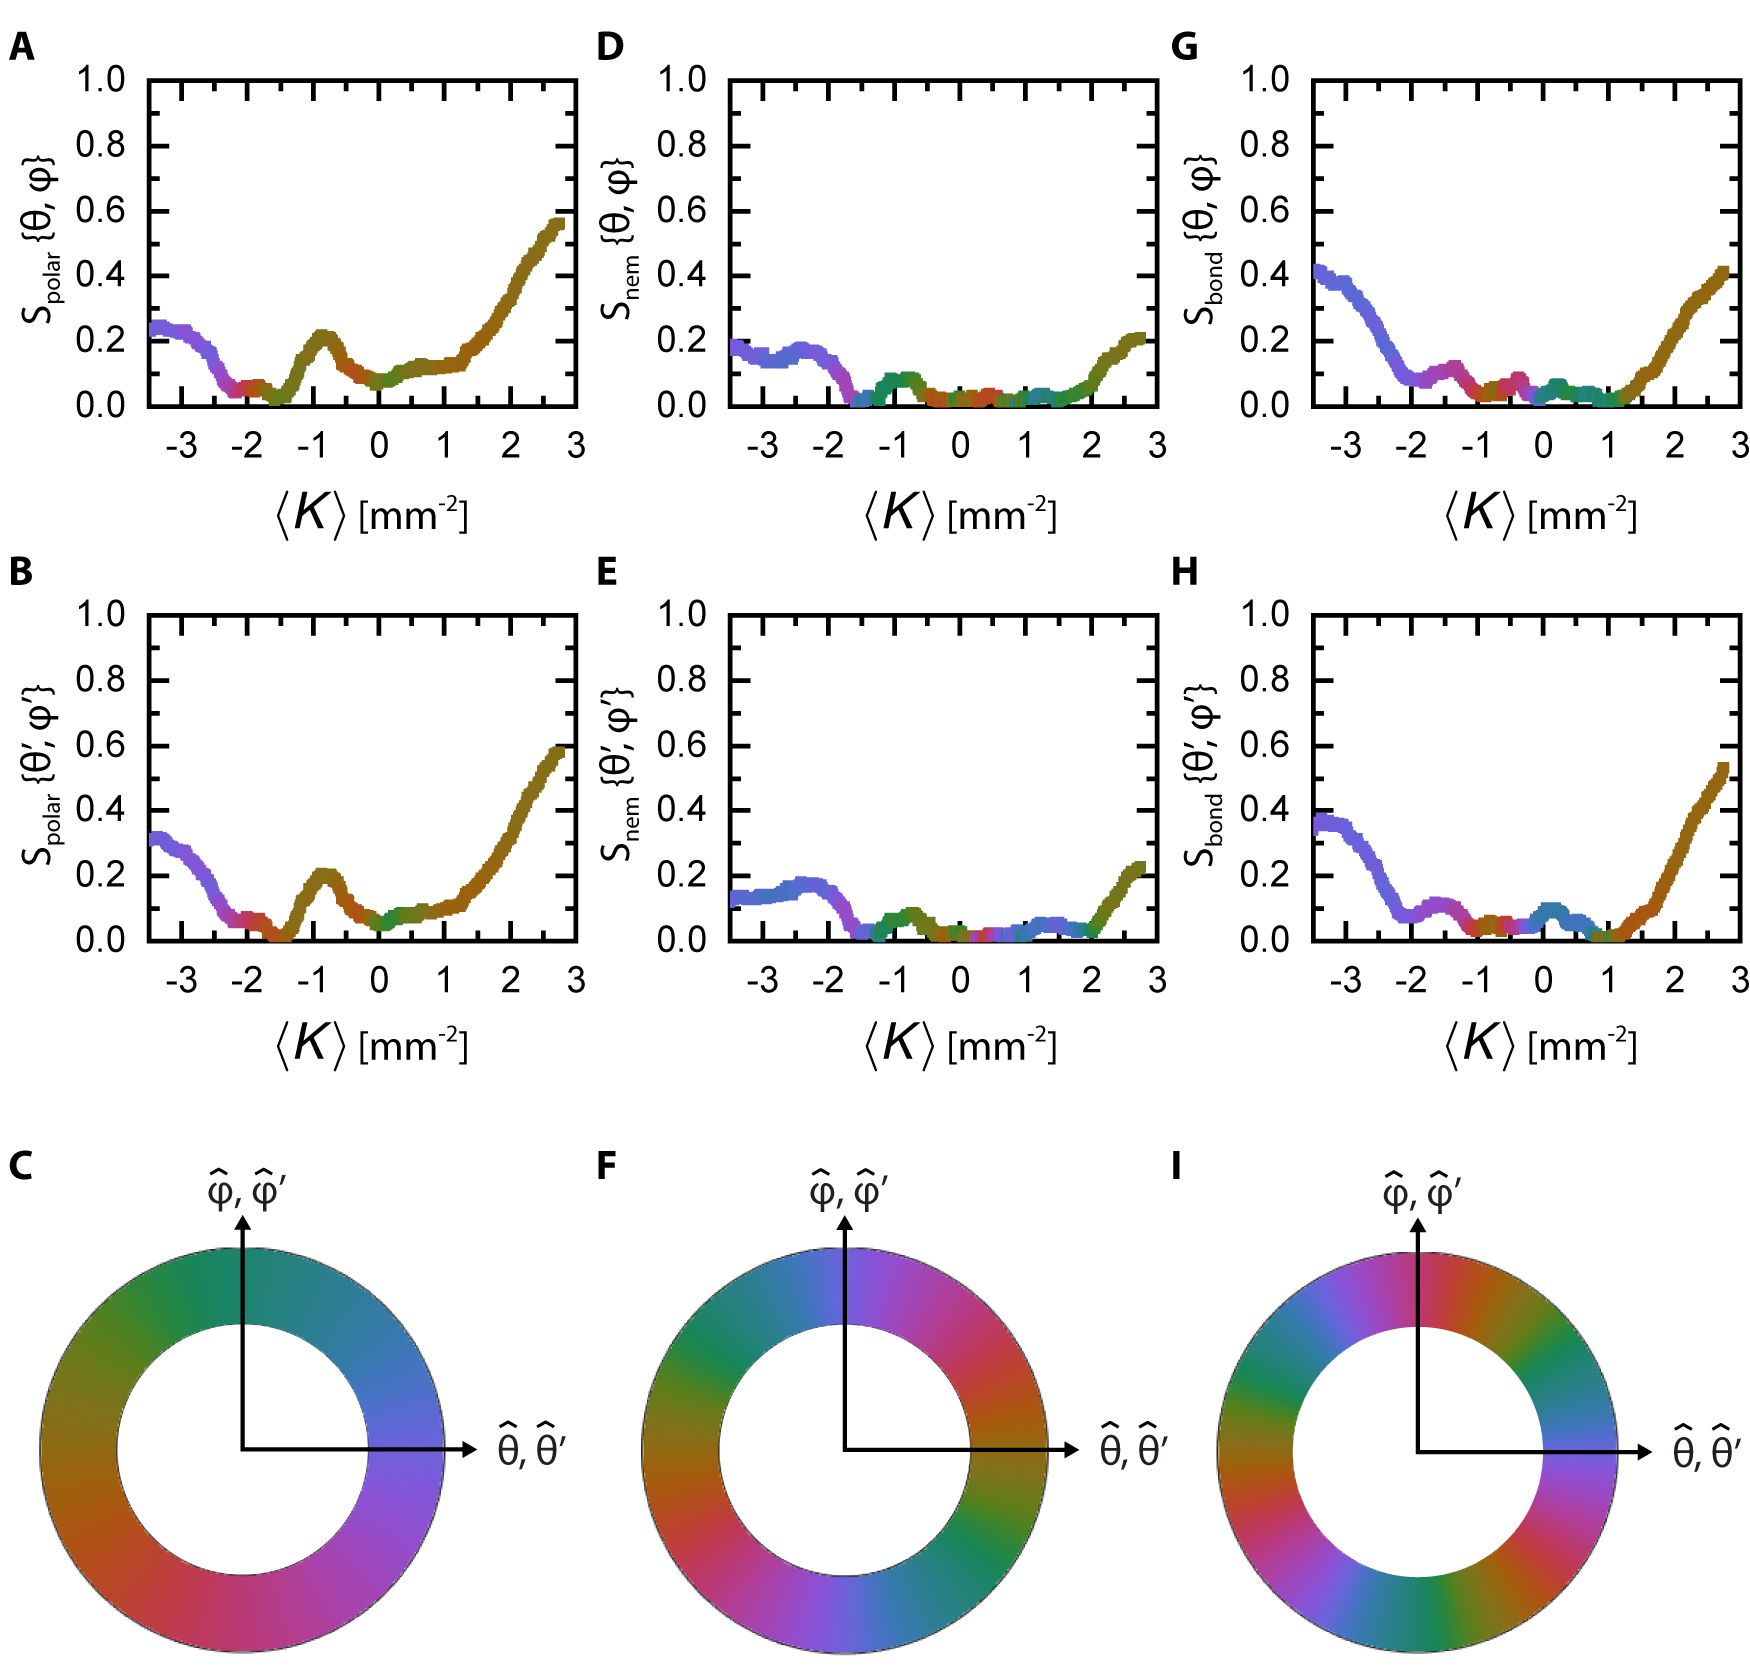
\includegraphics{figures/C7/Ch7-Figs_Orient_MeanK.png}
  \caption{[[COLROS WRONG]]$s = \pm 1/2$ defect ordering on a toroid with $\xi = 2.4$, $a = 268$ $\upmu$m, and an ATP concentration of 144 $\upmu$M.
  Magnitude and direction of (A--C) polar and (D--F) nematic order calculated for the $s = +1/2$ defects and (G--I) three-fold bond angle order calculated for the $s = -1/2$ defects.
  The order in (A,D,G) and (B,E,H) is calculated for the $\{\theta,\varphi \}$ and the $\{\nabla K = \theta',\varphi' \}$ coordinate systems, respectively, with (C,F,I) indicating the color scales used to denote orientation.
  }\label{f:7-Orient_MeanK}
\end{figure}\fxnote{colors wrong in figure.}

For an example toroid with with $\xi = 2.4$, $a = 268$ $\upmu$m, and an ATP concentration of 144 $\upmu$M, we plot the magnitude and orientation of the nematic and polar order for the $s = +1/2$ defects and the three-fold bond order for the $s = -1/2$ defects as a function of the mean Gaussian curvature in each bin  in Figure~\ref{f:7-Orient_MeanK}(A--C), Figure~\ref{f:7-Orient_MeanK}(D--F), and Figure~\ref{f:7-Orient_MeanK}(H--J) respectively.
We see that for both the $\{\Theta,\varphi\}$ [Figure~\ref{f:7-Orient_MeanK}(A,D,G)] and the $\{ \nabla K = \theta',\varphi' \}$ [Figure~\ref{f:7-Orient_MeanK}(B,E,H)] coordinate systems, the $s = \pm 1/2$ defects exhibit order in the regions where the magnitude of $K$ is larger.
Interestingly, we note that the $s = +1/2$ defects exhibit polar order on our toroidal droplets, rather than nematic order seen in flat space~\cite{RN27}.
Since we consider the defects at all time points when calculating the order, Figure~\ref{f:7-Orient_MeanK} reflects a persistent steady state.
In addition, the we see that the direction of the order is different in regions of negative and regions of positive Gaussian curvature.
In regions where $K > 0$, the $s = +1/2$ defects align along $-\hat{\theta}$, consistent with the idea that the $s = +1/2$ defects migrate towards $\theta = \pi$ in order to minimize their contribution to the free energy.
However, in regions where $K < 0$, the $s = +1/2$ defects align along $\hat{\theta}$, the opposite of what we expect; this indicates that on average, $s = +1/2$ defects in regions near the hold of the torus move further towards $\theta = 0$.
We note that even if the $s = +1/2$ defects want to move towards the hole, this is still consistent with curvature-induced defect unbinding provided that the $s = -1/2$ defects migrate towards the hole at a higher rate than the $s = +1/2$ defects.
Repeating this analysis for the remainder of our toroids, our preliminary results indicate that the $s = +1/2$defects posses steady state polar order, the $s = -1/2$ defects posses steady state three-fold bond angle order, and that the magnitude of the order grows with increasing $|K|$ for both defect species.

To investigate the origin of this order, we plot the polar order for the $s = +1/2$ defects and the three-fold bond angle order for the $s = -1/2$ defects against the mean defect density and against the mean $|K|$ in each bin in Figure~\ref{f:7-Orient_PolarHex}(A--D) and Figure~\ref{f:7-Orient_PolarHex}(F--I), respectively.
We see from the plotting the order against the mean defect density in each bin, that the magnitude of the order grows as the defect density decreases [polar order, Figure~\ref{f:7-Orient_PolarHex}(A.C) and three-fold bond angle order, Figure~\ref{f:7-Orient_PolarHex}(F,H)]; this is the opposite of the results in flat space~\cite{RN27}.
We also see that the magnitude of the defect order grows with increasing $|K|$ [polar order, Figure~\ref{f:7-Orient_PolarHex}(B,D) and three-fold bond angle order, Figure~\ref{f:7-Orient_PolarHex}(G,I)]; this makes intuitive sense as the gradient of the Gaussian curvature reflects the change in the ``background charge'' influencing the defects.
\begin{figure}
  \centering
  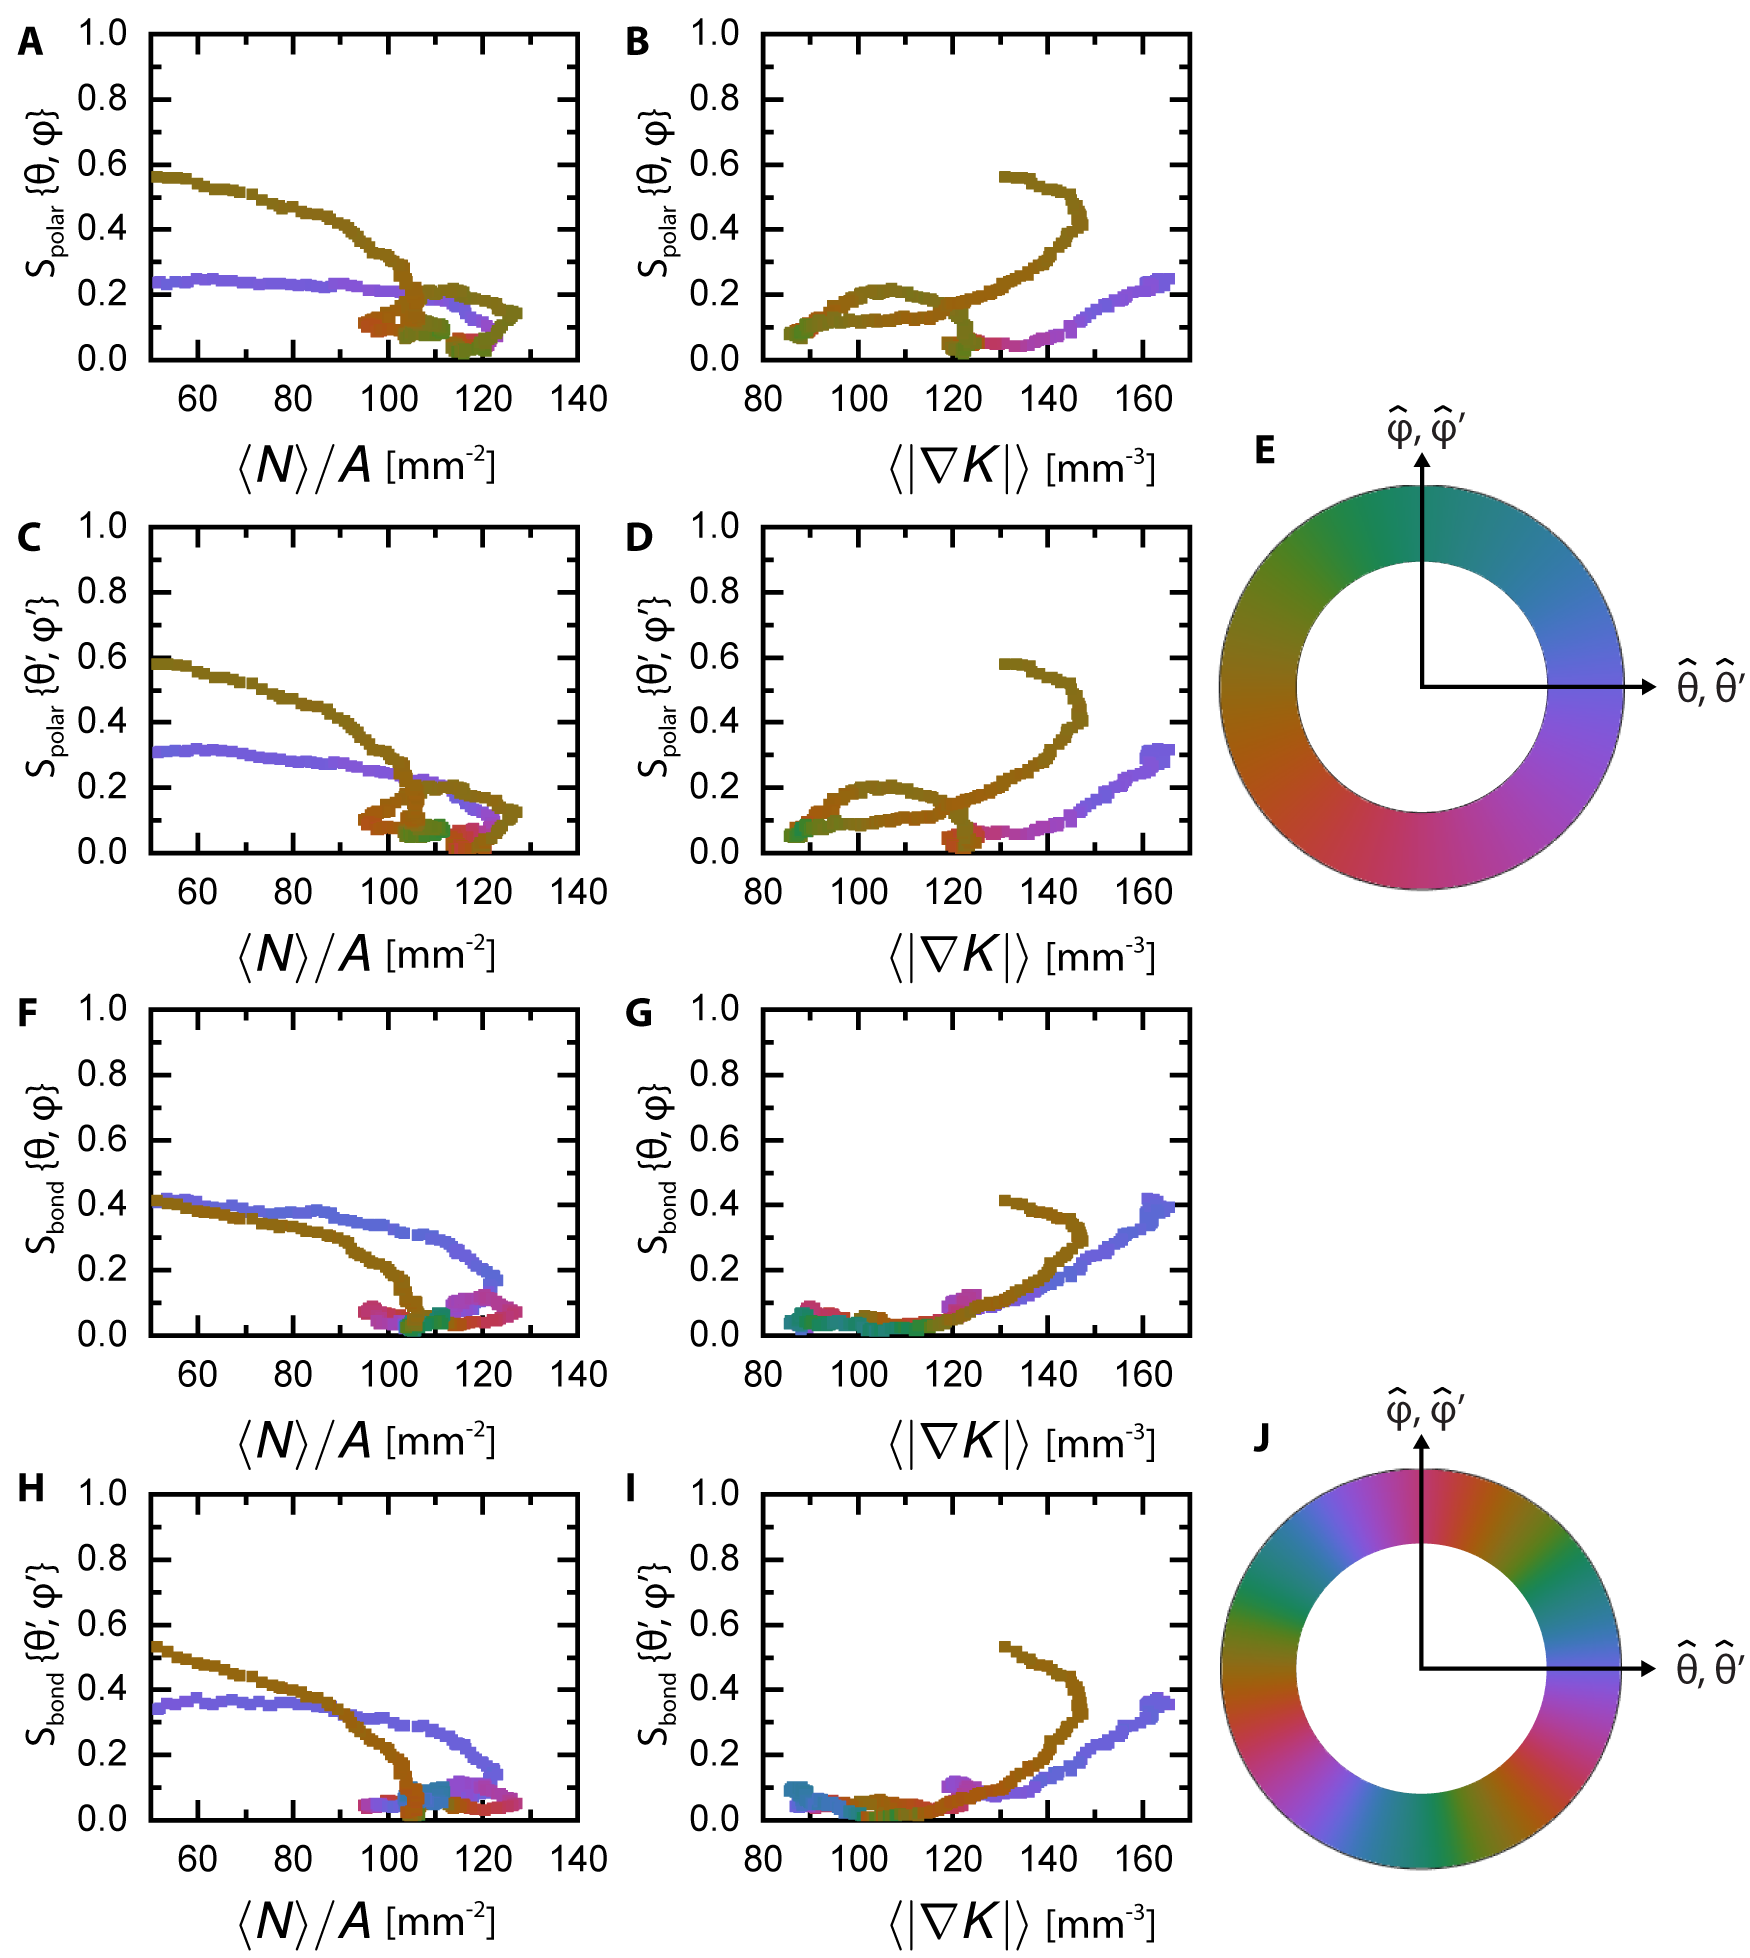
\includegraphics{figures/C7/Ch7-Figs_Orient_PolarHex.png}
  \caption{[[COLROS WRONG]]$s = \pm 1/2$ defect order plotted as a function of the mean defect density and of the magnitude of the gradient of the Gaussian curvature.
  Magnitude and direction of the (A--D) polar order for the $s = +1/2$ defects and the (F--I) three-fold bond angle order for the $s = -1/2$ defects.
  (A,B) and (F,G) are calculated in the $\{\theta,\varphi \}$ coordinate system, while (C,D) and (H,I) are calculated in the $\{ \nabla K = \theta',\varphi' \}$ coordinate system.
  The magnitude and direction of the order are plotted in (A,C,F,H) and (B,D,G,I) as a function of the mean defect density and of the mean magnitude of the gradient of the Gaussian curvature, respectively.
  The polar and three-fold bond angle color scales are displayed in (E,J), respectively.
  }\label{f:7-Orient_PolarHex}
\end{figure}\fxnote{colors wrong in figure.}


\subsection{Future Work}
To understand the nature of the ordering on the toroidal droplets, we need more data that focuses on the regions of the toroids that have a large Gaussian curvature magnitude.
These regions are where we see the ordering arise and where we have the least amount of data.
We are currently taking more data that looks specifically at these highly curved regions.
In addition, we are currently taking data on cylindrical surfaces in order to better understand how the global properties of a surface affect the defect ordering.
In addition, now that we see that there is a persistent steady-state in the defect orientations, we are analyzing smaller time windows to obtain the fluctuations in the orientation.

We also wish to understand defect orientation correlations in space at a given time.
To do this, we need to be able to calculate discrete geodesics on the surface of the torus.
We are currently working on implementing the algorithms in Refs.~\cite{RN322,RN323}.



\section{Determining the saddle-splay elastic constant: current status}
\subsection{Prior estimates in tori}
\subsection{Results from spherical drops}
\subsection{Distinguishing $K_{24}$ and surface contributions using twist angle and temperature}
